
\section{Phần cứng thực nghiệm \label{section_overview_propsed_method}}
\subsection{Cảm biến \label{section_overview_propsed_method}}

Trong quá trình ngủ, các chuyển động thân thể chủ yếu là chuyển động 
chậm, với biên độ nhỏ và không mang tính đột ngột. 
Các chuyển động thân thể chủ yếu mang tính chậm và thường xảy ra 
trong giai đoạn ngủ không chuyển động mắt nhanh (NREM), 
khi cơ thể có khả năng tự do thay đổi tư thế. Ngược lại, 
trong giai đoạn ngủ REM, hiện tượng ức chế trương lực cơ khiến 
cơ thể gần như bất động.
Do đó, việc ghi 
nhận chính xác các thay đổi tư thế ngủ đòi hỏi cảm biến có độ nhạy cao, 
khả năng phân giải tốt và ổn định với nhiễu nền thấp. Như đã trình bày 
trong Chương I, các cảm biến gia tốc MEMS sử dụng nguyên lý điện dung 
hiện đang được ứng dụng rộng rãi trong giám sát tư thế và chuyển động 
khi ngủ nhờ vào đặc điểm nổi bật là kích thước nhỏ gọn, tiêu thụ năng 
lượng thấp, tần số lấy mẫu phù hợp và đặc biệt là độ nhạy cao với 
chuyển động cường độ thấp.

Trong nghiên cứu của Vu và cộng sự (2023), dữ liệu tư thế ngủ được thu 
thập thông qua một thiết bị đeo đặt tại vùng bụng của người tham gia. 
Thiết bị này tích hợp cảm biến gia tốc ba trục ADXL345, 
bộ điều khiển ESP8266 và pin Lithium, tất cả được đóng gói trong 
một hộp nhựa nhỏ gọn \cite{vu2023}. Trong nghiên cứu của Boiko 
và cộng sự, cảm biến gia tốc ba trục ADXL355z 
được sử dụng để thu nhận tín hiệu hô hấp từ vùng ngực và bụng, 
với tần số lấy mẫu 62 Hz. Đây là cảm biến có độ nhiễu thấp, 
độ trôi nhiệt nhỏ và phù hợp với các ứng dụng y sinh. Trước đó, 
dòng cảm biến này cũng đã được ứng dụng thành công trong các phép 
đo tim–phổi \cite{Boiko2023}. Dữ liệu từ ADXL355z được đối chiếu với tín hiệu chuẩn 
thu từ dây đeo hô hấp của hệ thống SOMNO HD eco PSG, nhằm đảm bảo 
độ chính xác trong đánh giá tín hiệu sinh lý trong khi ngủ.
Trong nghiên cứu của Abdulsadig và cộng sự, dữ liệu gia tốc được 
thu thập bằng bo mạch điện tử thiết kế riêng tích hợp cảm biến gia tốc 
ba trục LIS2DH12 (STMicroelectronics) và vi điều khiển nRF5232 
(Nordic Semiconductor) \cite{Sleep_Posture_Detection}.


Dựa trên khảo sát thực tế và đánh giá các tiêu chí kỹ thuật phù hợp 
với đặc thù đo chuyển động chậm khi ngủ, luận văn lựa chọn hai dòng 
cảm biến gia tốc phổ biến là LIS3DH và LSM6DS3, đều do hãng 
STMicroelectronics sản xuất. Cả hai cảm biến đều tích hợp khả năng đo gia tốc ba trục, 
hỗ trợ các chuẩn giao tiếp \texttt{I\textsuperscript{2}C} và \texttt{SPI}, 
đồng thời có thể hoạt động trong chế độ tiêu thụ điện năng siêu thấp (\textit{ultra-low power mode}), 
đáp ứng yêu cầu sử dụng lâu dài trong các thiết bị đeo cá nhân hoạt động liên 
tục suốt đêm.

Trong các ứng dụng theo dõi tư thế ngủ, độ nhạy của cảm biến là một 
trong những tiêu chí quan trọng hàng đầu, bởi nó quyết định khả năng 
phát hiện các chuyển động nhỏ đặc trưng với biên độ thấp và tốc độ 
thay đổi chậm. Cảm biến \textbf{LIS3DH} cho phép lập trình dải đo động 
từ $\pm2g$ đến $\pm16g$, mang lại tính linh hoạt cao trong thiết kế hệ 
thống. Tuy nhiên, khi mở rộng dải đo, độ nhạy và độ phân giải sẽ giảm 
đáng kể. Ví dụ, đối với cảm biến 16-bit, nếu cấu hình ở dải $\pm100g$, 
độ phân giải chỉ đạt khoảng $0{,}003g$/LSB, điều này có thể làm suy giảm 
khả năng nhận biết các chuyển động vi mô trong khi ngủ - một yếu tố 
then chốt trong phân loại chính xác tư thế ngủ.




\begin{figure}[!ht]
		\centering
 		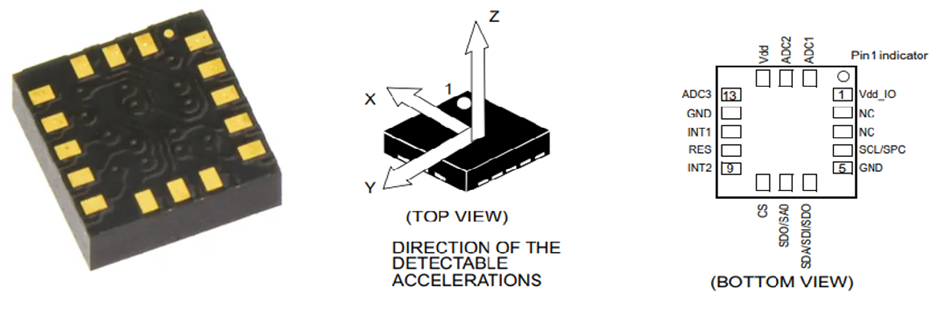
\includegraphics[width=0.8\textwidth]{images/lis.png}
		\caption{Cảm biến gia tốc LIS3DH và sơ đồ chân kết nối}
		\label{lis}
\end{figure}




\subsection{Vi xử lý}

Với sự phát triển vượt bậc và đa dạng của công nghệ chế tạo, 
có rất nhiều cấu hình phần cứng được nhiều nhóm tác giả lựa chọn phù 
hợp với các mục đích khác nhau. Trong đó, \cite{p_1} các tác giả đã 
sử dụng máy tính đơn Raspberry Pi kết hợp các điện trở cảm biến 
lực để phát hiện 4 tư thế ngủ với sự lấy nhãn từ video theo dõi người 
bệnh trong suốt quá trình lấy mẫu. Kwasnicki và cộng sự đã phát triển 
hệ thống ngủ có thể đeo (wearable sleep system) sử dụng bộ xử lý công 
suất thấp TI MSP430 và mô-đun RF Chipcon CC2420 cho truyền thông không 
dây kết hợp với cảm biến gia tốc 3 trục ADXL330, con quay hồi chuyển 
InvenSense ITG-3200, Honeywell HMC5843 để đo từ trường xác định 99.5\% 
chính xác 4 tư thế ngủ \cite{kwasnicki2018}. Tuy nhiên, các thiết bị vẫn 
yêu cầu một nguồn nặng lượng khiến cho tính liên tục bị hạn chế đáng kể. 
I.Yun và cộng sự đã phát triển thiết bị theo dõi tư thế ngủ của trẻ nhỏ 
sử dụng vi xử lý ATmega328P-PU cùng module Bluetooth kết hợp cảm biến gia 
tốc ADXL335 được đặt trên bụng đã nhưng lựa chọn về mặt cấu hình thiết bị 
và chế tạo ra mạch cung cấp năng lượng cho những thành phần cần thiết 
\cite{p_3}. Từ đó, giảm thiếu đáng kể mức tiêu thụ năng lượng và vẫn 
giữ nguyên độ chính xác nhưng khá bất tiện cho trẻ nhỏ. 
Trong nghiên cứu của Abdulsadig và cộng sự, 
hệ thống thu thập dữ liệu được xây dựng dựa trên một bo mạch tùy chỉnh tích 
hợp vi điều khiển nRF5232 (Nordic Semiconductor) – một SoC thuộc dòng 
ARM Cortex-M4F, hỗ trợ truyền thông không dây thông qua giao 
thức Bluetooth Low Energy (BLE). Vi điều khiển này đảm nhiệm đồng 
thời cả việc lấy mẫu dữ liệu từ cảm biến gia tốc ba trục LIS2DH12 
(STMicroelectronics) với tần số 100 Hz và truyền dữ liệu không dây 
theo thời gian thực \cite{Sleep_Posture_Detection, abdulsadig2023}. 
Trong nghiên cứu của Vũ Hoàng Diệu và cộng sự, 
mô-đun ESP32 được lựa chọn làm đơn vị xử lý trung tâm nhờ tích hợp bộ vi điều khiển hiệu năng cao, 
kết nối không dây Wi-Fi và khả năng mở rộng linh hoạt \cite{vu2023}. 
Với thiết kế nhỏ gọn, chi phí hợp lý và mức tiêu thụ điện năng thấp, 
ESP32 đáp ứng tốt yêu cầu của hệ thống thu thập dữ liệu tư thế ngủ theo 
thời gian thực. Thiết bị không chỉ cho phép truyền dữ liệu trực tiếp 
lên máy chủ hoặc nền tảng đám mây thông qua Wi-Fi, mà còn hỗ trợ 
lưu trữ cục bộ trên thẻ nhớ microSD, đảm bảo tính liên tục và 
an toàn dữ liệu trong điều kiện mất kết nối mạng.

Tuy nhiên, qua phân tích các nghiên cứu trên có thể thấy rằng phần 
lớn các cấu hình phần cứng hiện tại hoặc có chi phí triển khai cao, 
hoặc tiêu tốn năng lượng, hoặc gặp giới hạn trong khả năng tích hợp mô 
hình học máy tại thiết bị. Do đó, việc lựa chọn một kiến trúc vi xử lý 
vừa đảm bảo hiệu suất xử lý tín hiệu sinh lý thời gian thực, vừa tối 
ưu năng lượng và có khả năng triển khai mô hình TinyML là cần thiết. 
Trong số các kiến trúc hiện nay, dòng ARM Cortex-M4 nổi bật nhờ tính 
cân bằng giữa hiệu năng, mức tiêu thụ năng lượng thấp và khả năng hỗ 
trợ xử lý tín hiệu số, phù hợp với các hệ thống đeo được trong theo 
dõi tư thế ngủ.


Kiến trúc ARM có nhiều dòng vi xử lý khác nhau, được phát triển và nâng
cấp liên tục nhằm đáp ứng nhu cầu đa dạng trong lĩnh vực công nghệ nhúng. 
Trong đó, dòng Cortex-M thuộc kiến trúc ARMv7 đã trở thành nền tảng phổ 
biến cho các hệ thống nhúng sử dụng vi điều khiển nhờ vào hiệu suất cao, 
khả năng mở rộng và mức tiêu thụ năng lượng tối ưu. Dòng Cortex-M bao 
gồm nhiều phiên bản như Cortex-M0, Cortex-M0+, Cortex-M1, Cortex-M3, 
Cortex-M4 và Cortex-M7, mỗi phiên bản được thiết kế để phục vụ cho các mức 
độ yêu cầu hiệu năng khác nhau \cite{arm_cortex_m_comparison}. 
Các vi xử lý thuộc họ Cortex-M chủ yếu được ứng dụng trong các hệ thống 
nhúng thời gian thực, nơi yêu cầu sự cân bằng giữa hiệu suất xử lý, tiêu 
thụ năng lượng và chi phí. Một số vi xử lý ARM khác, không thuộc họ 
Cortex-M, được sử dụng trong các thiết bị hiệu suất cao như điện thoại 
thông minh và máy tính bảng, vốn yêu cầu cấu hình phần cứng mạnh hơn và 
khả năng xử lý đa tác vụ cao hơn.
Theo tài liệu \cite{cortexM4}, vi xử lý Cortex-M4 là một bộ xử lý 32-bit 
sử dụng kiến trúc tập lệnh rút gọn (RISC), được xây dựng theo kiến trúc 
Harvard, trong đó bus dữ liệu và bus lệnh được tách biệt nhằm tối ưu 
hiệu suất truy xuất bộ nhớ. Vi xử lý này hỗ trợ đầy đủ cả tập lệnh 
Thumb-1 (16-bit) và Thumb-2 (hỗn hợp 16/32-bit), mang lại sự linh hoạt 
trong mã hóa lệnh và tiết kiệm không gian bộ nhớ chương trình.

Về hiệu năng, Cortex-M4 đạt từ 1,25 đến 1,95 DMIPS/MHz (Dhrystone Million Instructions Per Second per MHz), cho thấy khả năng xử lý hiệu quả trong các ứng dụng nhúng yêu cầu độ chính xác và độ phản hồi thời gian thực cao. Bên cạnh đó, vi xử lý hỗ trợ tối đa 240 tín hiệu ngắt, bao gồm cả ngắt không thể bị chặn (Non-Maskable Interrupts – NMI), cùng khả năng cấu hình từ 8 đến 256 mức ưu tiên ngắt, giúp hệ thống hoạt động ổn định trong môi trường có nhiều sự kiện cạnh tranh đồng thời.
Ngoài ra, hiện nay ứng dụng trí tuệ nhân tạo (AI) tại thiết bị biên (Edge AI) đang ngày càng phổ biến, đặc biệt trong các lĩnh vực như nhà thông minh, thiết bị đeo, giám sát an ninh và công nghiệp 4.0. Với khả năng xử lý tín hiệu số (DSP) và hỗ trợ các mạng nơ-ron nhỏ gọn, các vi xử lý Cortex-M, đặc biệt là dòng Cortex-M4, đang được khai thác để triển khai các mô hình học sâu nhẹ (tinyML) ngay trên vi điều khiển \cite{electronics11162545}\cite{applicationCortexM4}.


\begin{figure}[!ht]
		\centering
 		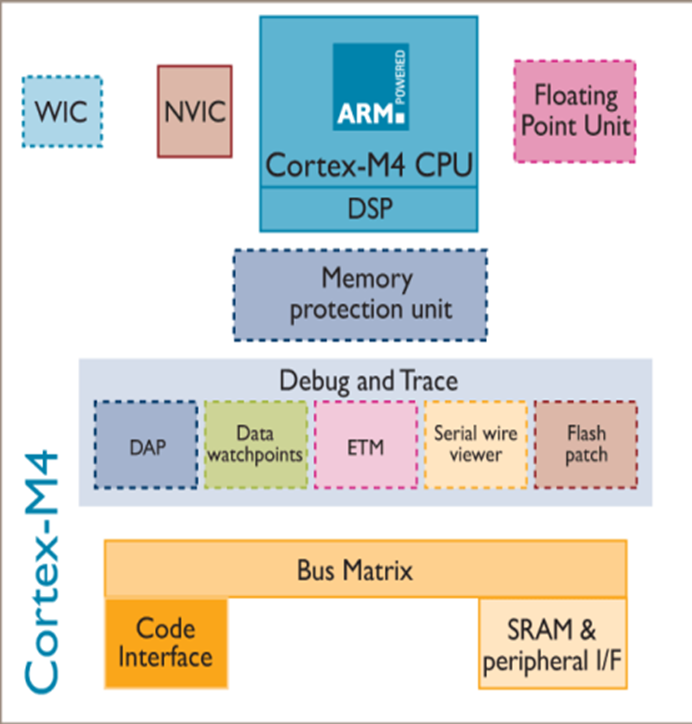
\includegraphics[width=0.8\textwidth]{images/cortexM4.png}
		\caption{Thành phần chính của vi điều khiển Cortex-M4}
		\label{cortexM4}
\end{figure}

Kết nối bus được mô tả trong Hình~\ref{cortexM4} cho phép truyền dữ liệu đồng thời trên nhiều bus khác nhau, đồng thời cung cấp khả năng quản lý truyền dữ liệu hiệu quả, chẳng hạn như sử dụng bộ đệm ghi và điều khiển hướng bit hoạt động (bit-banding). Hệ thống cũng có thể bao gồm các cầu bus (bus bridges) nhằm kết nối nhiều loại bus vào một mạng duy nhất sử dụng chung không gian bộ nhớ. Ngoài ra, bộ xử lý được trang bị hệ thống hỗ trợ gỡ lỗi tích hợp, bao gồm khả năng kiểm soát gỡ lỗi, thiết lập điểm ngắt (breakpoint) chương trình và điểm theo dõi dữ liệu (watchpoint). Khi xảy ra sự kiện gỡ lỗi, hệ thống có thể tạm dừng trạng thái hoạt động của lõi xử lý để phục vụ việc phân tích và xử lý lỗi.

Bên cạnh đó, kiến trúc Cortex-M4 tích hợp Bộ điều khiển ngắt vectored lồng nhau (Nested Vectored Interrupt Controller – NVIC) với khả năng hỗ trợ lên đến 240 tín hiệu yêu cầu ngắt, bao gồm cả ngắt không chắn được (NMI). NVIC hỗ trợ xử lý ngắt lồng nhau một cách tự động bằng cách so sánh mức ưu tiên giữa các yêu cầu ngắt với mức ưu tiên hiện tại đang được xử lý.

Đối với các ứng dụng yêu cầu tiết kiệm năng lượng, hệ thống còn được trang bị bộ đánh thức ngắt (Wake-up Interrupt Controller – WIC), cho phép đưa bộ vi điều khiển vào chế độ nghỉ bằng cách tắt hầu hết các thành phần không cần thiết, đồng thời duy trì khả năng đánh thức hệ thống khi phát hiện một yêu cầu ngắt. Ngoài ra, cơ chế bảo vệ bộ nhớ cũng được tích hợp nhằm đảm bảo an toàn cho hệ thống, ví dụ như chỉ cho phép truy cập đọc tại một số vùng bộ nhớ hoặc ngăn người dùng truy cập vào các vùng dữ liệu đặc quyền của hệ điều hành hoặc ứng dụng hệ thống.


\begin{figure}[!ht]
		\centering
 		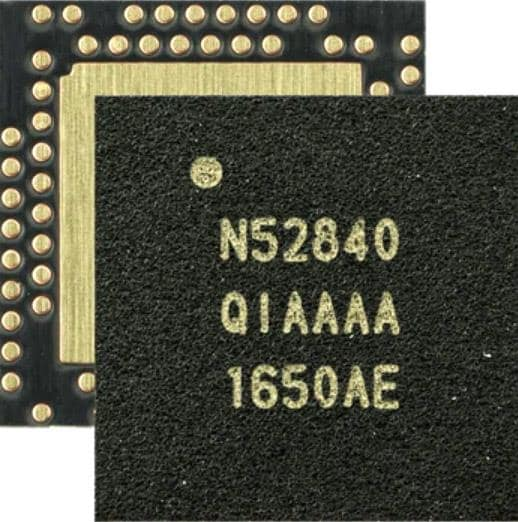
\includegraphics[width=0.8\textwidth]{images/NRF52840-QFA_SPL.jpg}
		\caption{Nordic Semiconductor NRF52840}
		\label{lis}
\end{figure}
Sau quá trình khảo sát và so sánh các dòng vi xử lý phổ biến, tác giả 
lựa chọn nRF52840 (Nordic Semiconductor) làm nền tảng phần cứng cho hệ 
thống đề xuất, nhờ vào các ưu điểm nổi bật như kích thước nhỏ, 
tiêu thụ năng lượng thấp và tích hợp sẵn giao tiếp Bluetooth Low Energy 
(BLE). Đây là vi xử lý cao cấp nhất trong dòng nRF52, thuộc loại hệ thống 
trên một vi mạch (System-on-Chip – SoC), được thiết kế chuyên biệt cho 
các ứng dụng không dây tầm ngắn và tiết kiệm năng lượng \cite{nrf52840}.

\textbf{nRF52840} tích hợp bộ thu phát đa giao thức hoạt động ở băng tần 2.4 GHz 
và bộ xử lý trung tâm Arm Cortex-M4F chạy ở xung nhịp 64 MHz, 
kèm bộ xử lý dấu phẩy động (FPU). Vi xử lý này được trang bị bộ nhớ 
1 MB Flash và 256 KB RAM, hỗ trợ chuẩn Bluetooth 5.3 cùng khả năng giao 
tiếp đa giao thức (multiprotocol), cho phép cải thiện tốc độ, phạm vi 
truyền và độ tin cậy của kết nối không dây. Hệ thống bảo mật tích hợp 
đầy đủ, bao gồm các tính năng mã hóa phần cứng, đáp ứng yêu cầu khắt khe 
về bảo vệ dữ liệu. Ngoài khả năng hoạt động trong dải điện áp rộng 
từ +1.7 V đến +5.5 V (tương thích với nguồn pin và USB), nRF52840 còn 
cung cấp các giao tiếp ngoại vi phong phú: tối đa hai giao diện I2C, 
bốn SPI master, ba SPI slave, bốn kênh PWM hỗ trợ EasyDMA, cùng với 
năm bộ định thời 32-bit, phù hợp cho các ứng dụng đòi hỏi xử lý thời 
gian thực chính xác. Tất cả các đặc điểm trên khiến nRF52840 trở thành 
lựa chọn lý tưởng cho các hệ thống nhúng đeo được tích hợp AI nhẹ và 
kết nối không dây thông minh.

Ngoài ra, nRF52840 hỗ trợ một hệ sinh thái phần mềm mạnh mẽ, bao gồm SDK 
của Nordic và nền tảng TensorFlow Lite for Microcontrollers, giúp rút 
ngắn thời gian phát triển và triển khai hệ thống TinyML. Thiết bị còn 
sở hữu khả năng quản lý năng lượng linh hoạt, tương thích tốt với nguồn pin hoặc USB. 





\subsection{Bluetooth năng lượng thấp}

Với mục tiêu tối ưu hóa năng lượng và đảm bảo khả năng hoạt động lâu dài 
cho thiết bị đeo sử dụng pin, Bluetooth Low Energy (BLE) được lựa chọn 
làm chuẩn kết nối không dây chính trong hệ thống phần cứng.

\begin{figure}[!ht]
		\centering
 		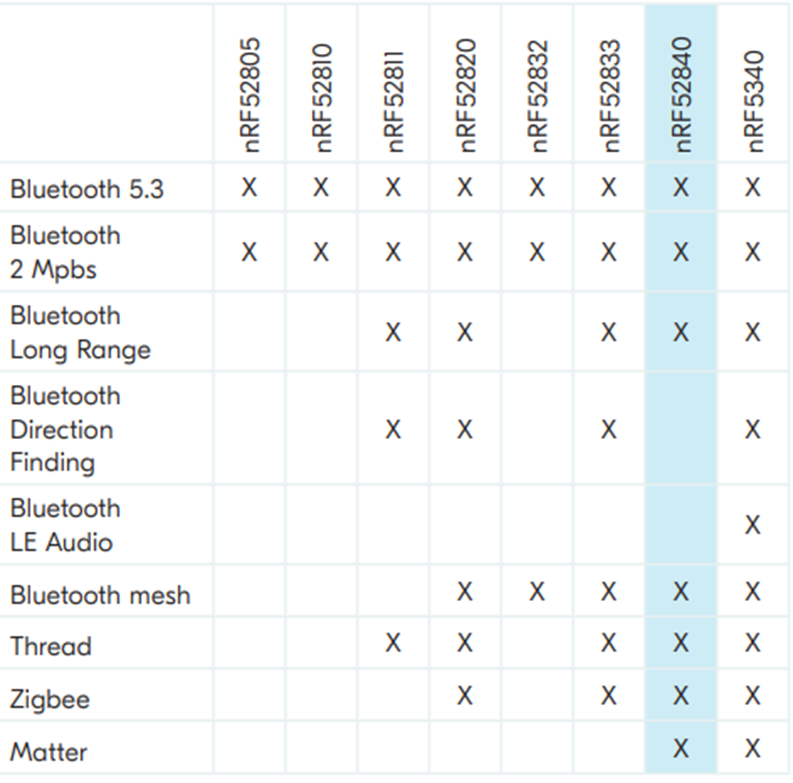
\includegraphics[width=0.8\textwidth]{images/ble.png}
		\caption{Các kiểu kết nối không dây trong họ chip nRF52}
		\label{ble}
\end{figure}

BLE là giao thức kết nối không dây được thiết kế chuyên biệt cho 
các ứng dụng năng lượng thấp, hoạt động ở băng tần ISM 2.4 GHz, 
hỗ trợ thông lượng ứng dụng lên đến 1.4 Mbps. Với ưu thế tiêu thụ năng 
lượng tối thiểu nhưng vẫn đảm bảo tốc độ truyền phù hợp, BLE đặc biệt 
thích hợp cho các thiết bị y sinh hoạt động liên tục bằng pin có dung 
lượng hạn chế. BLE hiện được hỗ trợ phổ biến trên hầu hết các hệ điều 
hành như iOS, Android, macOS, Windows 10 và Linux, cũng như trong các 
thiết bị di động hiện đại.

Về mặt bảo mật, BLE tích hợp các cơ chế mã hóa và xác thực nhằm đảm bảo 
tính bí mật, toàn vẹn và riêng tư của dữ liệu truyền qua mạng. 
Công nghệ này đã trở thành một phần tiêu chuẩn trong hầu hết các 
thiết bị di động hiện đại như smartphone, máy tính bảng, và laptop, 
đồng thời được hỗ trợ đầy đủ trên các hệ điều hành phổ biến bao gồm iOS, 
Android, macOS, Windows 10 và Linux. Bluetooth 5 là bước phát triển 
đột phá tiếp theo kể từ khi BLE được giới thiệu trong chuẩn Bluetooth 
4.0, mang đến hàng loạt cải tiến đáng kể giúp mở rộng phạm vi ứng dụng 
và nâng cao hiệu suất hệ thống. Một trong những cải tiến nổi bật là 
chế độ 2 Mbps, cho phép tăng gấp đôi tốc độ truyền lý thuyết, tương 
ứng với thông lượng thực tế lên đến 1.4 Mbps. Quan trọng hơn, chế độ 
này còn giúp giảm đáng kể mức tiêu thụ năng lượng – cụ thể là giảm một 
nửa năng lượng tiêu thụ trên mỗi bit dữ liệu – từ đó kéo dài thời gian 
hoạt động của thiết bị hoặc cho phép sử dụng các nguồn năng lượng nhỏ 
và chi phí thấp hơn \cite{BLE}. 

Bên cạnh đó, tính năng Advertising Extensions (mở rộng quảng cáo) đã 
cách mạng hóa cơ chế phát sóng của BLE. Các gói quảng cáo giờ đây có 
thể chứa lượng dữ liệu gấp 8 lần so với phiên bản trước, cho phép 
truyền tải các khối dữ liệu lớn hơn mà không cần thiết lập kết nối 
ngay lập tức. Đồng thời, các gói quảng cáo có thể được xâu chuỗi 
để tạo thành các tập tin quảng cáo phức hợp. Tính năng lựa chọn kênh 
được tối ưu hóa giúp tăng cường độ ổn định và khả năng chống nhiễu 
trong các môi trường có mật độ thiết bị cao. Đặc biệt, chế độ Long 
Range mở rộng đáng kể phạm vi truyền thông của BLE, cho phép các thiết 
bị duy trì kết nối trong toàn bộ không gian của một ngôi nhà thông minh 
hoặc trong các ứng dụng IoT công nghiệp quy mô vừa và nhỏ.




\begin{figure}[!ht]
	\centering
 	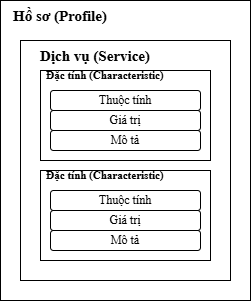
\includegraphics[width=0.5\textwidth]{images/gatt.drawio.png}
	\caption{Cấu trúc của GATT}
	\label{gatt}
\end{figure}

BLE tổ chức logic giao tiếp dựa trên mô hình GATT 
(Generic Attribute Profile). GATT quy định cách hai thiết bị BLE 
trao đổi dữ liệu thông qua các đơn vị logic: dịch vụ (services) 
và đặc tính (characteristics). Giao thức nền tảng là Attribute Protocol 
(ATT) – nơi mỗi đặc tính được định danh bằng UUID 16-bit hoặc 128-bit, 
với quyền truy cập như chỉ đọc, chỉ ghi, hoặc hỗ trợ thông báo (notify).

Một điểm quan trọng trong mô hình GATT là tính kết nối độc quyền: 
tại một thời điểm, thiết bị ngoại vi chỉ có thể duy trì một kết nối 
duy nhất với thiết bị trung tâm. Khi kết nối được thiết lập, thiết bị 
ngừng quảng cáo, điều này hạn chế khả năng kết nối đồng thời từ 
nhiều thiết bị.

Ngoài ra, vi xử lý nRF52840 còn hỗ trợ Bluetooth Mesh, cho phép thiết 
lập mạng lưới nhiều-nút (many-to-many), sử dụng BLE làm lớp truyền tải 
vật lý. Mỗi nút trong mạng có thể đóng vai trò chuyển tiếp (relay), 
cho phép dữ liệu lan truyền đến các vùng rộng hơn theo mô hình phân 
tán – phù hợp với các ứng dụng IoT quy mô lớn như nhà thông minh, 
chiếu sáng công nghiệp hoặc giám sát phân tán. Trong mạng Mesh, 
các gói dữ liệu có thể được đóng gói qua advertising packet hoặc 
qua các giao tiếp GATT tùy tình huống sử dụng.

Các profile BLE là tập hợp các dịch vụ được chuẩn hóa bởi Bluetooth 
SIG hoặc định nghĩa tùy chỉnh, ví dụ như dịch vụ UART tùy chỉnh gồm 
hai đặc tính RX và TX, tương ứng với kênh nhận và truyền.

\subsection{Thiết bị thực nghiệm}
Trong khuôn khổ của khóa luận, nhằm đảm bảo tiến độ triển khai và tính an 
toàn trong giai đoạn thử nghiệm, tác giả lựa chọn sử dụng bộ kit thương 
mại Adafruit Playground để tiến hành thực nghiệm sơ bộ. Bộ kit này tích 
hợp sẵn cảm biến gia tốc MEMS LIS3DH được gắn tại vị trí trung tâm, 
cho phép đo gia tốc theo ba trục không gian X, Y và Z với độ chính xác cao. 
Theo tài liệu từ nhà sản xuất, chi phí cho mỗi bộ kit Adafruit vào khoảng 
25 USD \cite{ada_overview}. Trong bộ kit, cảm biến LIS3DH được kết nối với 
vi điều khiển thông qua giao thức SPI, với chân chọn thiết bị (CS) được 
gán tại chân số 8 và đầu ra ngắt tùy chọn (IRQ) tại chân số 7 (IRQ \#4). 
Theo sơ đồ bố trí tiêu chuẩn của kit, trục X định hướng theo chiều giắc 
USB, trục Y hướng sang bên trái, và trục Z vuông góc theo hướng mặt trên 
của thiết bị.

Bên cạnh đó, để mở rộng khả năng nghiên cứu và đánh giá tính khả thi khi 
tích hợp học máy nhẹ (TinyML) cũng như kết nối không dây, nhóm nghiên 
cứu sử dụng thêm nền tảng Arduino Nano 33 BLE Sense. Đây là vi điều khiển 
hiện đại tích hợp vi xử lý nRF52840 (ARM Cortex-M4F), hỗ trợ Bluetooth 
Low Energy (BLE) và nhiều cảm biến tích hợp (IMU, microphone, nhiệt độ, 
độ ẩm, v.v.), đồng thời tương thích với nền tảng TensorFlow Lite for 
Microcontrollers \cite{nano33ble}.

Đáng chú ý, bên cạnh việc sử dụng các bộ kit sẵn có, một thành viên khác 
trong nhóm đang tiến hành phát triển và xây dựng bản mạch phần cứng 
tùy chỉnh dựa trên các thông số kỹ thuật đã được phân tích ở các phần 
trước. Hướng tiếp cận này không chỉ giúp nhóm triển khai nhanh chóng hệ 
thống thử nghiệm trong giai đoạn đầu, mà còn mở ra khả năng thiết kế một 
thiết bị nhúng chuyên dụng, tối ưu hơn về chi phí, hiệu năng và khả năng 
tích hợp trong các ứng dụng thực tiễn.


\begin{figure}[!ht]
		\centering
 		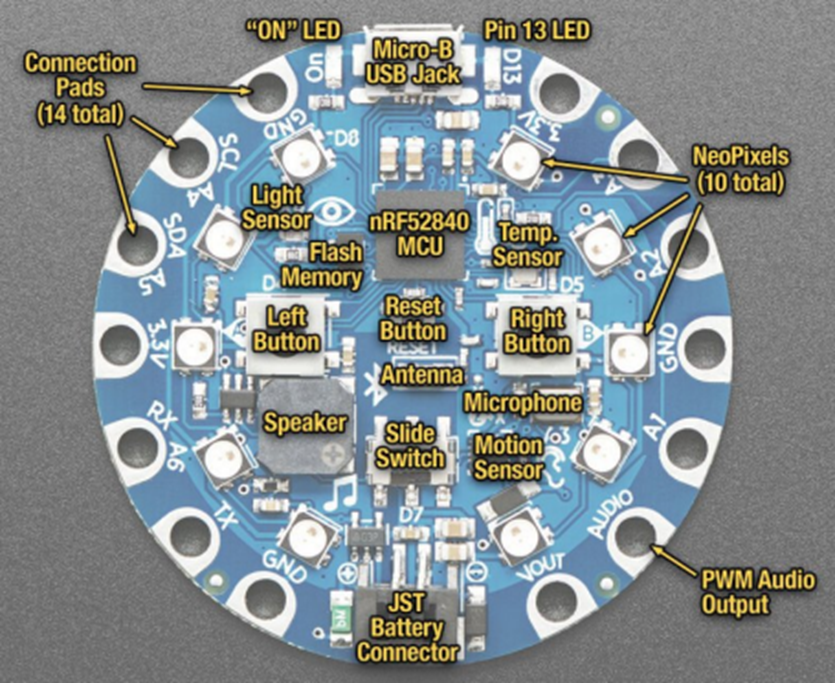
\includegraphics[width=0.8\textwidth]{images/detail_ada.png}
		\caption{Cấu trúc các thành phần trên Circuit PlayGround}
		\label{detail_ada}
\end{figure}





\section{Hệ thống thu thập, xử lý, lưu trữ dữ liệu}
Phần này trình bày tổng quan kiến trúc hệ thống bao gồm: 
lập trình firmware trên vi điều khiển để thu thập dữ liệu cảm biến, 
thiết kế ứng dụng di động làm cầu nối giữa phần cứng và hệ thống đám mây, 
cùng với backend và cơ sở dữ liệu lưu trữ phục vụ huấn luyện mô hình. 
Nội dung cũng đề cập đến các yêu cầu chức năng, phi chức năng và 
thiết kế hệ thống ở mức cao nhằm đảm bảo khả năng triển khai thực 
tế và mở rộng trong tương lai.

\subsection{Lập trình vi xử lý}

\begin{figure}[!]
		\centering
 		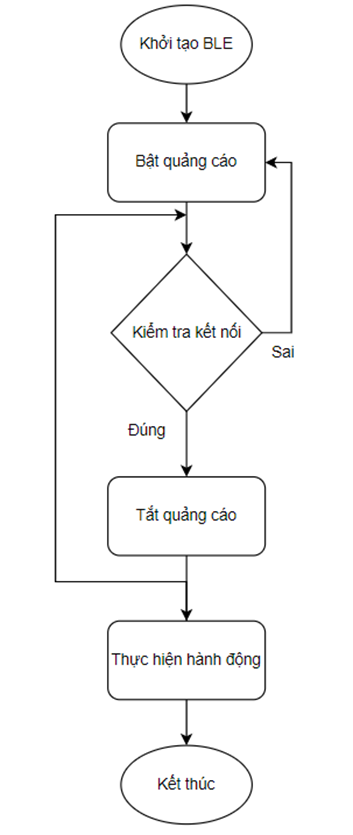
\includegraphics[width=0.5\textwidth]{images/flowBLE.png}
		\caption{Lưu đồ hoạt động của thiết bị BLE}
		\label{flowBLE}
\end{figure}

\begin{lstlisting}[float,language=C,caption=Tập lệnh khởi tạo và kết nối Bluetooth từ thư viện của AdaFruit, label=arduinoBLE,captionpos=b]
void startAdv(void)
{
  // Advertising packet
  Bluefruit.Advertising.addFlags(BLE_GAP_ADV_FLAGS_LE_ONLY_GENERAL_DISC_MODE);
  Bluefruit.Advertising.addTxPower();

  // Include HRM Service UUID
  Bluefruit.Advertising.addService(positionService);

  // Include Name
  Bluefruit.Advertising.addName();
  
  /* Start Advertising
   * - Enable auto advertising if disconnected
   * - Interval:  fast mode = 20 ms, slow mode = 152.5 ms
   * - Timeout for fast mode is 30 seconds
   * - Start(timeout) with timeout = 0 will advertise forever (until connected)
   * 
   * For recommended advertising interval
   * https://developer.apple.com/library/content/qa/qa1931/_index.html   
   */
  Bluefruit.Advertising.restartOnDisconnect(true);
  Bluefruit.Advertising.setInterval(32, 244);    // in unit of 0.625 ms
  Bluefruit.Advertising.setFastTimeout(30);      // number of seconds in fast mode
  Bluefruit.Advertising.start(0);                // 0 = Don't stop advertising after n seconds  
}
\end{lstlisting}



Tác giả thực hiện lập trình trên Arduino IDE và thư viện Circuit Playground. Trong phần khởi tạo (setup) các bản tin quảng cáo (advertising) sẽ được khởi tạo và được thực thi. Tiếp theo là cấu hình các hàm kết nối, ngắt kết nối, cấu hình chung \gls{GATT} Hình~\ref{flowBLE}.



Trong mã nguồn \ref{arduinoBLE}, hàm startAdv có nhiệm vụ khởi tạo tên, thêm các dịch vụ và bắt đầu quảng cáo cho thiết bị. Sau đó, cấu hình cho \gls{BLE} theo định dạng \gls{GATT} sẽ được thiết lập. Đầu tiên, khởi tạo dịch vụ $positionService$ có mã định dang duy nhất(Universally Unique IDentifier - UUID) là 0x1821. Tiếp theo, thêm các đặc tính $BLE-GATT-UNIT-ACCELERATION
-METRES-PER-SECOND-SQUARED
$ và $BLE-GATT-UNIT-ANGULAR-ACCELERATION
-RADIAN-PER-SECOND-SQUARED
$ có UUID lần lượt là 0x2713 và 0x2744. Hàm cấu hình setupPosition được tác giả sử dụng để cấu hình chi tiết GATT cho BLE. Có 2 service được khởi tạo là gia tốc và con quay hồi chuyển. Tuy nhiên, trong khuôn khổ khóa luận tác giả tập trung vào giá trị gia tốc của cảm biến gia tốc. 


\begin{lstlisting}[float,language=C,caption=Tập lệnh khởi tạo các thuộc tính GATT, label=gattBle,captionpos=b]
void setupPosition(void)
{
 
  positionService.begin();

  accelerometerCharacter.setProperties(CHR_PROPS_NOTIFY+CHR_PROPS_READ+CHR_PROPS_WRITE );
  accelerometerCharacter.setPermission(SECMODE_OPEN, SECMODE_NO_ACCESS);
  accelerometerCharacter.setFixedLen(9);
  accelerometerCharacter.setCccdWriteCallback(cccd_callback);  // Optionally capture CCCD updates
  accelerometerCharacter.begin();
  uint8_t accelerometerData[9] = { 0b00000000, 0b00000000, 0b00000000,0b00000000,0b00000000,0b00000000,0b00000000,0b00000000,0b00000000}; // Set the characteristic to use 8-bit values, with the sensor connected and detected
  accelerometerCharacter.write(accelerometerData, 9);

  gyroscopeCharacter.setProperties(CHR_PROPS_READ);
  gyroscopeCharacter.setPermission(SECMODE_OPEN, SECMODE_NO_ACCESS);
  gyroscopeCharacter.setFixedLen(1);
  gyroscopeCharacter.begin();
  gyroscopeCharacter.write8(2);    // Set the characteristic to 'Wrist' (2)
}

\end{lstlisting}


\begin{lstlisting}[float,language=C,caption=Gửi dữ liệu từ BLE, label=sendBle,captionpos=b]
void setupPosition(void)
{
 
  positionService.begin();

  accelerometerCharacter.setProperties(CHR_PROPS_NOTIFY+CHR_PROPS_READ+CHR_PROPS_WRITE );
  accelerometerCharacter.setPermission(SECMODE_OPEN, SECMODE_NO_ACCESS);
  accelerometerCharacter.setFixedLen(9);
  accelerometerCharacter.setCccdWriteCallback(cccd_callback);  // Optionally capture CCCD updates
  accelerometerCharacter.begin();
  uint8_t accelerometerData[9] = { 0b00000000, 0b00000000, 0b00000000,0b00000000,0b00000000,0b00000000,0b00000000,0b00000000,0b00000000}; // Set the characteristic to use 8-bit values, with the sensor connected and detected
  accelerometerCharacter.write(accelerometerData, 9);

  gyroscopeCharacter.setProperties(CHR_PROPS_READ);
  gyroscopeCharacter.setPermission(SECMODE_OPEN, SECMODE_NO_ACCESS);
  gyroscopeCharacter.setFixedLen(1);
  gyroscopeCharacter.begin();
  gyroscopeCharacter.write8(2);    // Set the characteristic to 'Wrist' (2)
}

\end{lstlisting}


\textbf{setProperties} - phương thức để thay đổi thuộc tính liên quan đến quyền BLE có thể được đặt thành một hoặc nhiều lựa chọn sau:

\begin{itemize}
    \item CHR\_PROPS\_BROADCAST = bit (0)
    
    \item CHR\_PROPS\_READ = bit (1)
    
    \item CHR\_PROPS\_WRITE\_WO\_RESP = bit (2)
    
    \item CHR\_PROPS\_WRITE = bit (3)
    
    \item CHR\_PROPS\_NOTIFY = bit (4)
    
    \item CHR\_PROPS\_INDICATE = bit (5)
\end{itemize}
Ngoài ta còn nhiều hàm như \textbf{setPermission} để cài đặt tính bảo mật. \textbf{setFixedLen} để cấu hình gửi bao nhiêu bit.





\begin{figure}[!]
		\centering
 		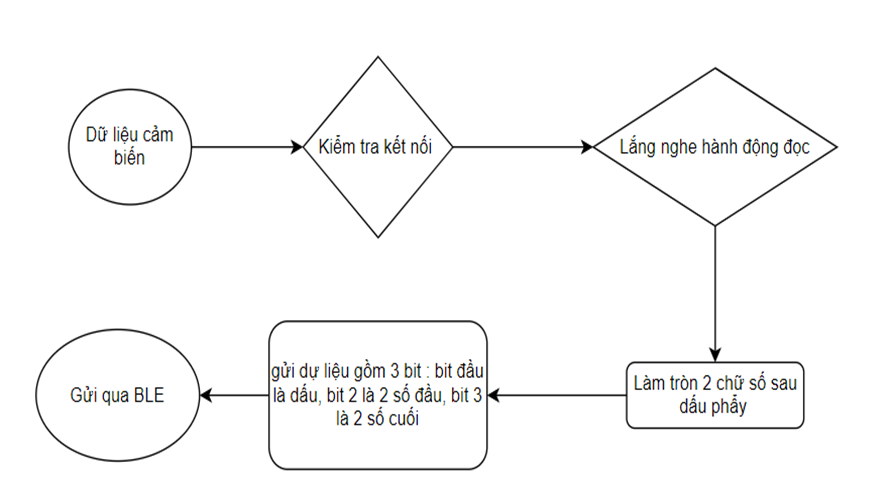
\includegraphics[width=1\textwidth]{images/sendBleFlow.png}
		\caption{Lưu đồ luồng gửi thông tin BLE}
		\label{sendBleFlow}
\end{figure}


















\subsection{Hiệu chuẩn cảm biến}
Việc thu nhận dữ liệu và tiền xử lý dữ liệu là cần thiết trong các hệ đo. Cảm biến mặc dù đã được hiệu chuẩn tại nơi sản xuất nhưng vẫn cần được hiệu chuẩn trong hệ thống và môi trường đo thực tế. Mục đích của việc hiệu chuẩn là cải thiện hiệu năng của cảm biến bằng cách loại bỏ hoặc giảm thiểu sai số trong dữ liệu đầu ra cảm biến. Lỗi cảm biến phân làm 2 loại i) lỗi mặc định và ii) lỗi ngẫu nhiên. Để xử lý lỗi mặc định, tác giả tác giả sử dụng gia tốc trọng trường để hiệu chuẩn cảm biến. Giá trị một trục gia tốc của cảm biến xoay lên trên so với mặt phẳng ngang sẽ nhận giá trị là -1g, khi xoay xuống dưới nhận giá trị là +1g. Hiệu chuẩn cảm biến bằng cách xoay cảm biến tạo bởi 6 vị trí tĩnh. Phương pháp xoay cảm biến từ +1 g đến -1 g giúp ta thu được giá trị 0 g chính xác và tin cậy.
\begin{figure}[!]
		\centering
 		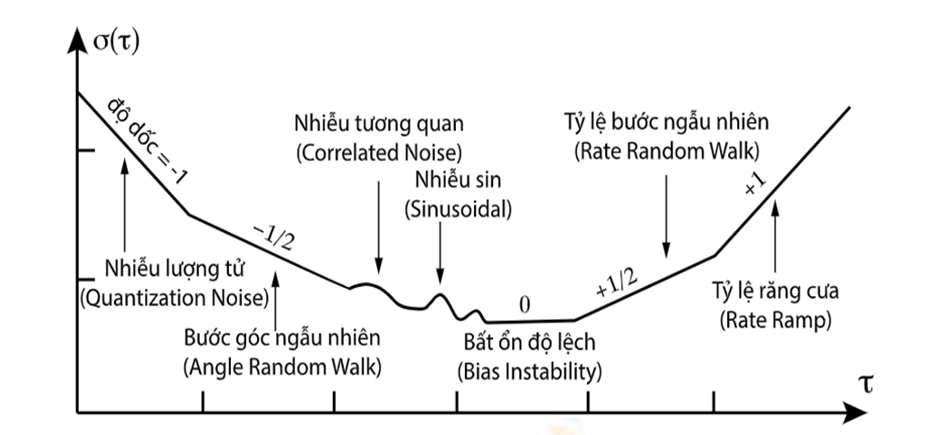
\includegraphics[width=1\textwidth]{images/allan.png}
		\caption{Minh hoạ kết quả phân tích đường cong Allan}
		\label{allan}
\end{figure}

\begin{figure}[!]
		\centering
 		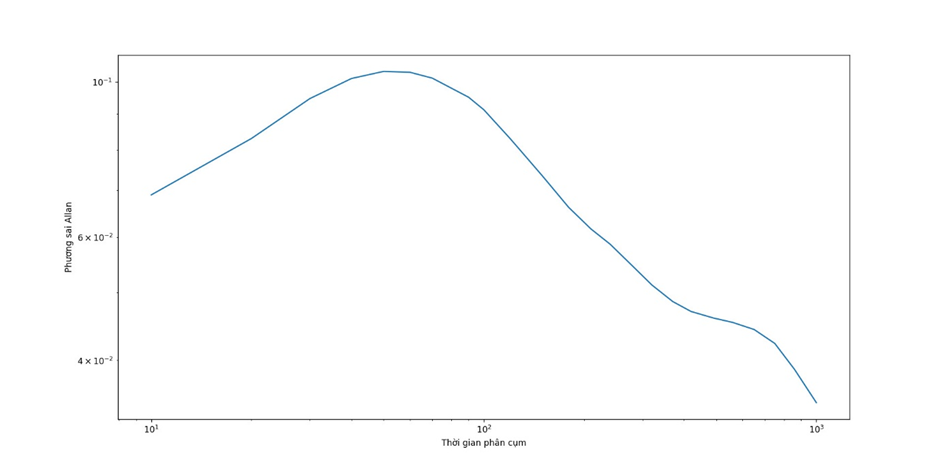
\includegraphics[width=1\textwidth]{images/allan_real.png}
		\caption{Biểu đồ phương sai Allan của trục x}
		\label{allan_real}
\end{figure}

Lỗi ngẫu nhiên phân tích theo phương sai Allan \cite{allan}. Phương sai Allan là phương pháp phân thích chuỗi dữ liệu trong miền thời gian để đo lường sự ổn định tần số trên miền tần số. Phương pháp này là một trong những phương pháp phổ biến nhất hiện nay để xác định và định lượng được nhiều loại nhiễu khác nhau tồn tại trong dữ liệu của cảm biến gia tốc, quán tính, cũng có thể sử dụng phương sai Allan để xác định các nhiễu nội tại trong một hệ thống như là một hàm trung bình cộng của thời gian. Các thành phần nhiễu cảm biến có thể xác định được bằng cách phân tích đồ thị log-log. Độ dốc đường cong Allan sẽ thể hiện các thành phần nhiễu khác nhau.

Tác giả thu tập được 1211210 mẫu dữ liệu khi để cảm biến đứng với tần số lấy mẫu là 10 Hz ở trong phòng với nhiệt độ bình thường. Kết quả đường cong Allan Hình \ref{allan_real} cho thấy nhiễu lượng tử xuất hiện chủ yếu là nhiễu lượng tử (Quantization noise) dựa trên việc đối chiếu hệ số góc với Hình \ref{allan_real}. Đây là nhưng nhiễu chủ yếu từ bản thân của cảm biến.


\begin{figure}[!]
		\centering
 		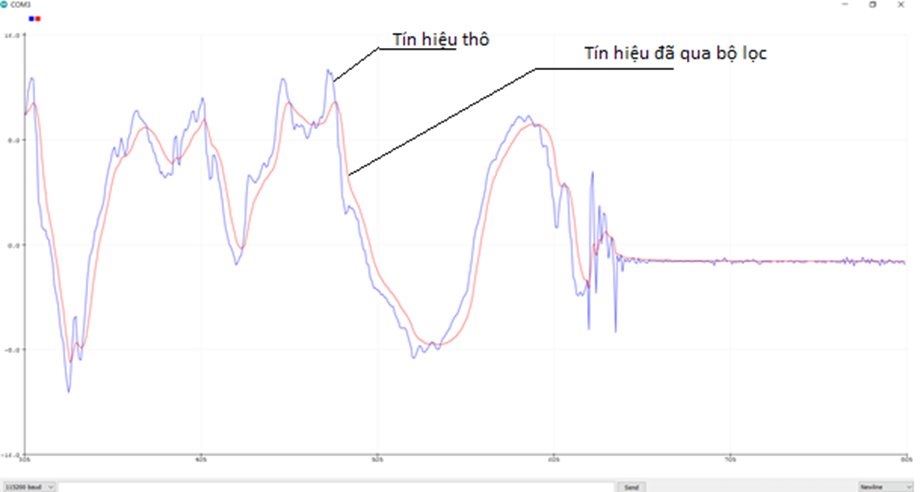
\includegraphics[width=1\textwidth]{images/kalman.png}
		\caption{Kết quả bộ lọc Kalman cho dữ liệu thô lấy trực tiếp từ trục X của cám biến gia tốc}
		\label{kalman}
\end{figure}
Trong khuôn khổ khoá luận, tác giả sử dụng bộ lọc Kalman để lọc các tín hiệu nhiễu đăc biệt là nhiễu lượng tử \cite{kalman}. Bộ lọc Kalman là thuật toán sử dụng chuỗi các giá trị đo lường, bị ảnh hưởng bởi nhiễu hoặc sai số, để ước đoán biến số nhằm tăng độ chính xác so với việc sử dụng duy nhất một giá trị đo lường. Bộ lọc Kalman là một bộ lọc đệ quy để ước lượng trạng thái của hệ thống tuyến tính, và cả hệ thống phi tuyến khi áp dụng phép ước lượng phi tuyến sang tuyến tính. Bộ lọc Kalman được ứng dụng rất nhiều trong lĩnh vực kĩ thuật, đặc biệt là lĩnh vực điều khiển. Tín hiệu sau khi được thu thâp sẽ được đi qua bộ lọc ở vi xử lý rồi mới được chuyển tới ứng dụng để hiển thị và lưu trữ. Bộ lọc đã được tác giả thực hiện lập trình và có kết quả như Hình ~\ref{kalman}. Kết quả cho thấy, bộ lọc Kalman đã lược bỏ dữ liệu ít ý nghĩa hoặc nhiễu (ồn) cho một đường biểu diễn mượt mà hơn.





\subsection{Xây dựng phần mềm ứng dụng}

Phần mềm ứng dụng được thiết kế với mục tiêu tạo thuận lợi cho người dung. Nhiệm vụ chính là thực hiện liên kết đến phần cứng và giao diện trực tiếp để người dùng thực hiện các thao tác. 

\begin{itemize}
    \item Ngôn ngữ: Dart
    
    \item Framework: Flutter
    
    \item Hệ điều hành: Android
    
    \item Kết nối với phần cứng: Ble
    
    \item Chức năng: Đảm bảo các yêu cầu cơ bản, thuận tiện cho người sử dụng.
\end{itemize}
\begin{figure}[!]
		\centering
 		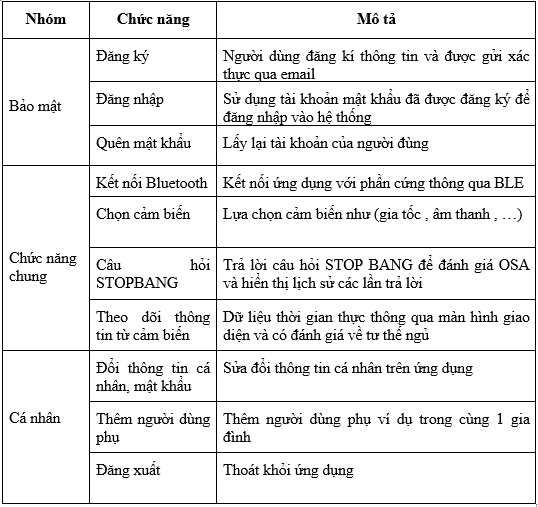
\includegraphics[width=1\textwidth]{images/app_flow.png}
		\caption{Các chức năng cơ bản của ứng dụng}
		\label{app_flow}
\end{figure}

Ứng dụng gồm 3 nhóm chức năng chính, Hình ~\ref{app_flow} bao gồm nhóm chức năng bảo mật, nhóm chức năng chung và nhóm chức năng cá nhân.
\begin{figure}[!]
		\centering
 		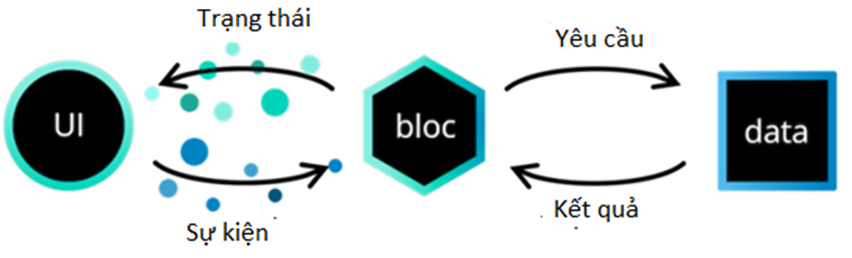
\includegraphics[width=0.8\textwidth]{images/flutter.png}
		\caption{Cấu trúc BLOC}
		\label{flutter}
\end{figure}


\begin{lstlisting}[float,language=dart,caption=Tập lệnh để tìm kiểm dịch vụ cảm biến ,label=flutterBle,captionpos=b]
StreamBuilder<List<BluetoothService>>(
      stream: device.services,
      initialData: [],
      builder: (c, snapshot) {
        if (snapshot.data!.length > 0) {
          isService = true;
        }
        BluetoothService serviceAcclerometer;
        if (snapshot.data == null || snapshot.data!.length == 0) {
          return Text("Please contact customer Service");
        }
        for (int i = 0; i < snapshot.data!.length; i++) {
          if (snapshot.data![i].uuid.toString() ==
              Constants.ACCLEROMETER_SERVICE) {
            accelerometerService = snapshot.data![i];
           }
        }
        if (accelerometerService == null) {
          return Text("Please contact customer Service");
        }
        for (int i = 0;
            i < accelerometerService!.characteristics.length;
            i++) {
          print(accelerometerService!.characteristics[i].uuid);
          if (accelerometerService!.characteristics[i].uuid
                  .toString() ==
              Constants.ACCLEROMETER_CHARACTION) {
            accelerometerCharactis =
                accelerometerService!.characteristics[i];
          }
        }
}));

\end{lstlisting}

\begin{lstlisting}[float,language=Java,caption=Tập lệnh đọc dữ liệu từ BLE, label=flutter_get_data,captionpos=b]
void setupPosition(void)
{
 
  positionService.begin();

  accelerometerCharacter.setProperties(CHR_PROPS_NOTIFY+CHR_PROPS_READ+CHR_PROPS_WRITE );
  accelerometerCharacter.setPermission(SECMODE_OPEN, SECMODE_NO_ACCESS);
  accelerometerCharacter.setFixedLen(9);
  accelerometerCharacter.setCccdWriteCallback(cccd_callback);  // Optionally capture CCCD updates
  accelerometerCharacter.begin();
  uint8_t accelerometerData[9] = { 0b00000000, 0b00000000, 0b00000000,0b00000000,0b00000000,0b00000000,0b00000000,0b00000000,0b00000000}; // Set the characteristic to use 8-bit values, with the sensor connected and detected
  accelerometerCharacter.write(accelerometerData, 9);

  gyroscopeCharacter.setProperties(CHR_PROPS_READ);
  gyroscopeCharacter.setPermission(SECMODE_OPEN, SECMODE_NO_ACCESS);
  gyroscopeCharacter.setFixedLen(1);
  gyroscopeCharacter.begin();
  gyroscopeCharacter.write8(2);    // Set the characteristic to 'Wrist' (2)
}

\end{lstlisting}



\textbf{Flutter} là cross-platform dành cho ứng dụng di động viết theo kiểu hướng đối tượng. Nó có thể lập trình cho cả ứng dụng trên nền tảng Android và IOS. Khả năng phát triển nhanh chóng có nhiều thành phần (Widget) có sẵn, đẹp, dễ sử dụng và có nhiều thư viện và cộng đồng sử dụng. Trong ứng dụng này tác giả sử dụng Bloc là một thư viện để quản lý trạng thái cho ứng dụng Flutter B.L.o.C (Business Logic Component). Nhận sự kiện như là đầu vào và trả về kết quả là trạng thái. Bloc được xây dựng dựa trên RxDart. Chúng ta có thể chia kiến trúc Flutter thành 3 lớp như Hình ~\ref{flutter}. Trong đó UI là giao diện của người dùng, nơi người dùng nhìn thấy dữ liệu, thao tác. Bloc là thư viện để quản lý các trạng thái của ứng dụng. Các sự kiện là các hành động như ấn nút, nhập dữ liệu, v.v.




Khi đã lấy được đối tượng tính năng (charactis instance), tác giả sẽ liên tục đẩy  hành động đọc (read) từ phần mềm ứng dụng đến vi điều khiển. Khi vi điều khiển nhận được hành động đọc được gửi từ ứng dụng sẽ trả lại tín hiệu của cảm biến. Ở đây, các BLE gửi các dữ liệu theo định dạng là mảng các phần tử có kiểu là UInt8. Do đó, sau khi nhận được dữ liệu từ phần cứng, dữ liệu dạng UInt8 được chuyển về dạng Number. Với quy trình như vậy, hệ thống có độ trễ rất thấp (real time). Cuối cùng việc lưu trữ thông tin cảm biến được thông qua giao thức Giao thức Truyền tải Siêu Văn Bản (Hyper Text Transfer Protocol - HTTP) truyền lên phía máy chủ(backend) và được thực hiện ở đoạn Mã \ref{flutter_get_data}.
\begin{lstlisting}[float,language=C,caption="Cấu trúc dữ liệu của phần nội dung đẩy lên máy chủ",label=format_ble,captionpos=b]
{
    "value": "0.88%0.66%0.99@2022-01-01/0.88%0.66%0.99@2022-01-01/0.88%0.66%0.99@2022-01-01",
    "customer": "62a5f5672ad9c724ef117d76"
}

\end{lstlisting}

Việc đẩy tín hiệu như vậy, tránh được tình trạng tắc nghẽn ở phía backend. Trong thời gian tới, cơ chế nghe/nhận (pub/sub) sẽ được áp dụng để tránh tình trạng gọi các yêu cầu (request) liên tục. Dữ liệu sẽ được đẩy lên theo định dạng Mã \ref{format_ble}:

Ngoài ra, tác giả phát triển thêm tính năng bộ câu hỏi STOPBANG nhằm đánh giá ban đầu người dùng. Và những dữ liệu này có trọng số quan trọng trong việc đánh giá chỉ số AHI sử dụng học máy sau này. Tính năng thêm người dùng được sử dụng để tránh phải thao tác tạo mới nhiều lần nhưng vẫn giữ được tính bảo mật, lấy lại dữ liệu khi mà quên tài khoản, mật khẩu.



\subsection{Thiết kế và xây dựng hệ thống lưu trữ   }
\begin{figure}[b!]
		\centering
 		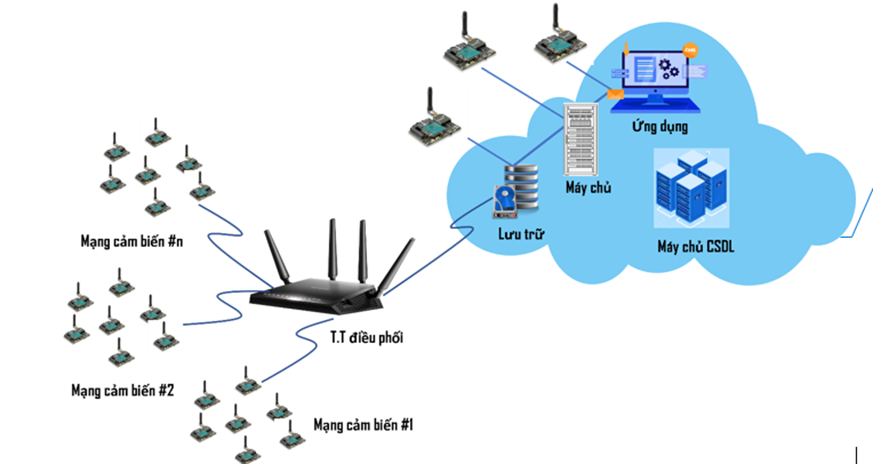
\includegraphics[width=0.8\textwidth]{images/cloud.png}
		\caption{Mô hình tích hợp giữa mạng cảm biến và cấu trúc dữ liệu đám mây}
		\label{cloud}
\end{figure}


Dữ liệu (data) là cơ sở của công nghệ trí tuệ nhân tạo để phân tích, đánh giá, dự đoán nhiều lĩnh vực trong cuộc sống. Vì mỗi thiết bị phần cứng chỉ có không gian bộ nhớ có hạn nên việc lưu trữ trên hệ thống đám mây (cloud) đang là phương pháp phổ biến nhất Hình ~\ref{cloud}. Việc triển khai dữ liệu lên cloud giúp xóa bỏ khoảng cách địa lý, thuận tiện cho việc trích xuất bất kì nơi nào miễn là có kết nối internet, qua đó có thể dễ dàng xuất ra các file text, csv và thuận tiện chia sẻ trao đổi với các nhóm nghiên cứu khác. Mục tiêu dài hạn của hướng nghiên cứu này là việc sử dụng cơ sở dữ liệu đủ lớn cho các mô hình toán học nhằm dự đoán, hỗ trợ ra quyết định trong các hoạt động sàng lọc và chẩn đoán chứng \gls{OSA} ở người. 


\begin{itemize}
    \item MongoDB được thiết kế để có thể truy vấn hiệu quả các bộ dữ liệu rất lớn, ngay cả khi dữ liệu được phân chia trên nhiều máy chủ, miễn là có thể chọn share key đoạn phù hợp khớp với các truy vấn đọc phổ biến nhất của mình.
    
    \item Hỗ trợ tốt đối với dữ liệu TimeStamp.
    
    \item Các chỉ mục được phân nhóm tối ưu hóa hiệu suất và lưu trữ chỉ mục.
    
    \item Tự động xóa dữ liệu cũ hơn. Lưu trữ dữ liệu bằng kho lưu trữ trực tuyến Atlas và dễ mở rộng
\end{itemize}


\begin{figure}[!]
		\centering
 		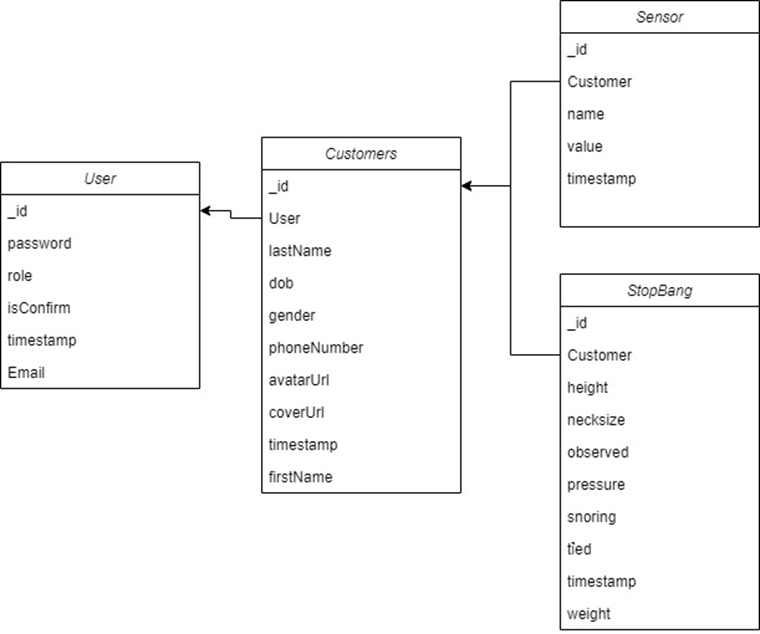
\includegraphics[width=1\textwidth]{images/csdl.png}
		\caption{Cấu trúc lưu trữ dữ liệu}
		\label{cloud}
\end{figure}
\begin{figure}[b!]
		\centering
 		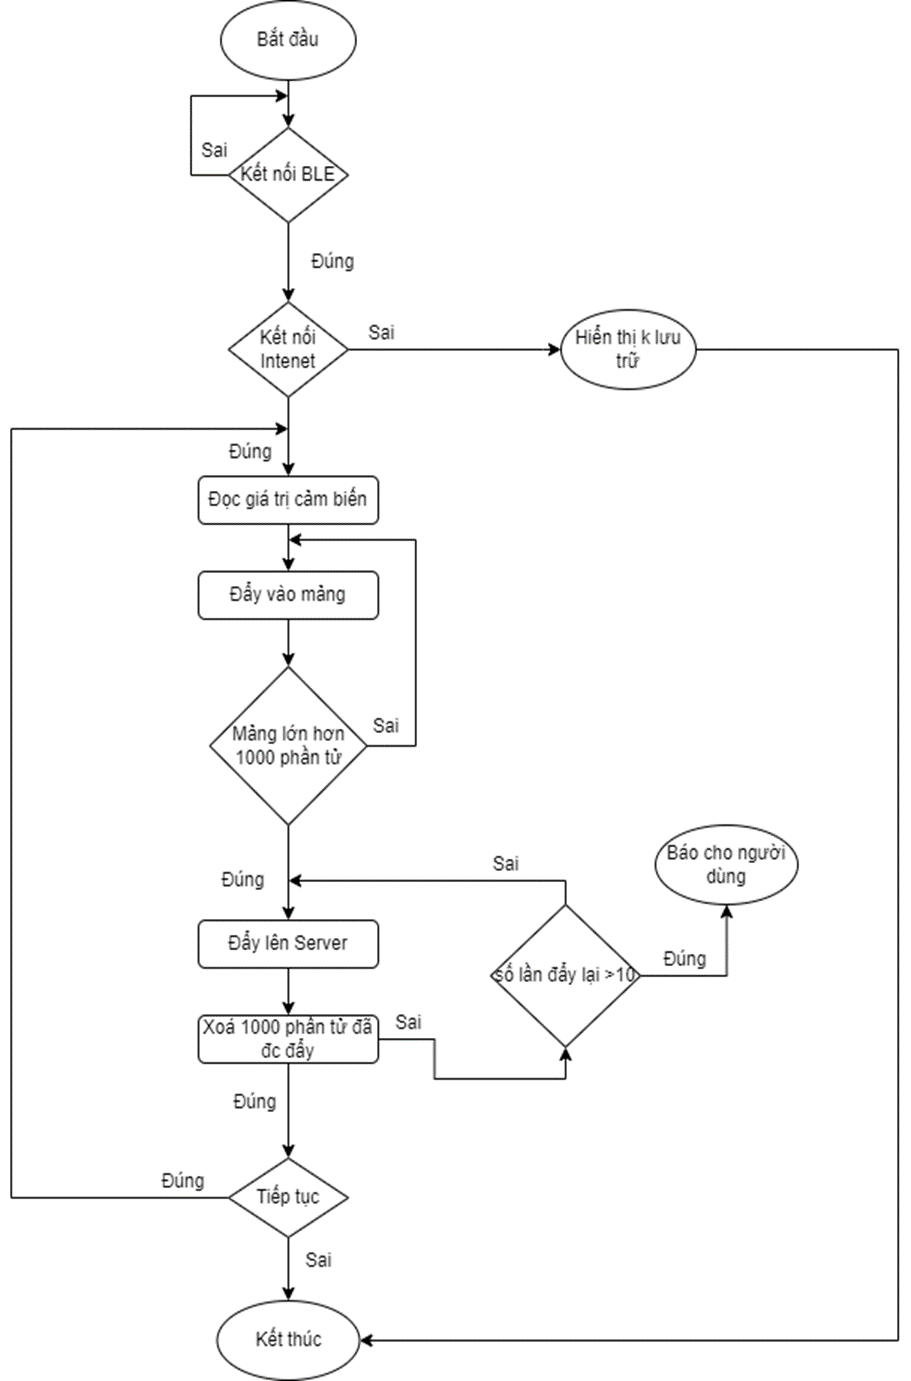
\includegraphics[width=0.9\textwidth]{images/flow_http.png}
		\caption{Lưu đồ thuật toán lưu trữ dữ liệu cảm biến}
		\label{flow_http}
\end{figure}


Trong khóa luận này, phần máy chủ của hệ thống được xây dựng trên nền tảng NodeJs và triển khai trên AWS - nền tảng đám mây cho phép các lập trình viên xây dựng, triển khai, quản lý và mở rộng ứng dụng. Cơ sở dữ liệu sử dụng trên nền tảng MongoDb Atlas hỗ trợ free 500Mb.

Để tránh tình trạng quá tải server khi có quá nhiều yêu cầu truy cập cùng lúc đến, tác giả đã gộp các giá trị cảm biến vào 1 mảng 1000 phần tử rồi đẩy mảng đó lên backend. Việc lưu trữ này yêu cầu phải xác định được chính xác thời gian của từng giá trị của biến số trên ứng dụng di động và truyền lên cùng giá trị của 3 trục x, y, z. Việc lưu trữ dữ liệu được tác giả mô tả như lược đồ, Hình ~\ref{flow_http} bao gồm 2 trường hợp:



\begin{itemize}
    \item Khi người dùng không có kết nối mạng thì người dùng chỉ được phép truy cập vào BLE và hiển thị dữ liệu không có lưu trữ.
    
    \item Khi trường hợp người dùng đã đăng nhập và có kết nối mạng thì ứng dụng sẽ tự động lưu trữ khi thu thập đủ 1000 giá trị. Nếu không thành công 10 lần sẽ báo cho người dùng.
\end{itemize}


\subsection{Tìm hiểu, ứng dụng phân loại tư thế ngủ bằng học máy  }

Tác giả cũng đã tìm hiểu nhiều mô hình, phương pháp để phân loại các tư thế ngủ, tư thế cơ bản của con người và đánh giá chỉ số AHI dự trên các tín hiệu cảm biến thu được. Các bước cơ bản để tiến hành dự án học máy liên quan đến các tín hiệu cảm biến:


\begin{figure}[b!]
		\centering
 		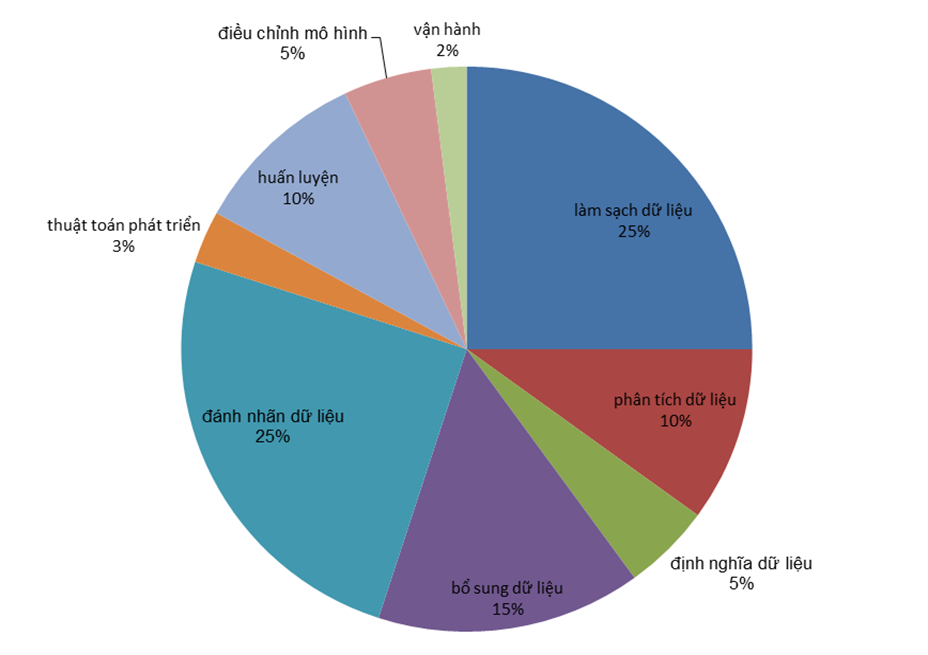
\includegraphics[width=1\textwidth]{images/hocmay_time.png}
		\caption{Phân bố thời gian sử dụng đối với dự án học máy}
		\label{hocmay_time}
\end{figure}

\begin{itemize}
    \item Thu thập dự liệu (bao gồm thu thập và gắn nhãn cho dữ liệu)
    
    \item Khám phá dữ liệu (đánh giá cân bằng dữ liệu, tỉ lệ dữ liệu có ý nghĩa)
    
    \item Chuẩn bị dữ liệu (làm sạch dữ liệu, tạo ra các đặc tính trên miền thời gian và miền tần số)
    
    \item Mô hình hoá dữ liệu (lựa chọn ra các mô hình phù hợp)
    
    \item Lựa chọn tính năng (lựa chọn ra các tính năng có ý nghĩa cao đối với mô hình)

    \item Tinh chỉnh mô hình
\end{itemize}

Jeng PY và cộng sự đã đề xuất chế tạo 2 thiết bị đeo ở cổ và ở cổ tay để đánh giá tư thế ngủ ở người \cite{Jeng}. Trong dự án này, tín hiệu thu được ở thiết bị đeo ở tay được chia thành những cửa sổ 1 giây rồi trích xuất các tính năng trên cửa sổ đó. Cảm biến đeo ở cổ sẽ được sử dụng để lấy nhãn tín hiệu theo phương pháp lấy đa số của tín hiệu trong cửa sổ. Nhóm tác giả đã sử dụng mô hình SVM và RF để đánh giá và đạt được kết quả có độ chính xác lần lượt là 82\% và 72\%. Nhóm của Saha S., Kabir M và cộng sự đã tiến hành nghiên cứu 1 thiết bị đeo được sử dụng bao gồm cảm biến gia tốc, cảm biến âm trên 31 đối tượng thử nghiệm. Sau đó họ tiến hành loại bỏ các bộ dữ liệu có độ dài dưới 2 giờ và cuối cùng sử dụng so sánh ngưỡng để xác định chứng OSA bằng việc phân chia các cửa sổ 10s với độ lặp 80\% \cite{Saha}. Trong khi đó, nhóm của Syeda Zuriat-e-Zehra Ali và cộng sử đã nghiên cứu và thử nghiệm thiết bị gối ngủ để tự điều chỉnh hoặc báo hiệu khi có chứng ngưng thở khi ngủ dựa trên các tín hiệu thô như nồng độ Oxi trong máu, nhịp tim [27]. Jarvis L, Moninger S và cộng sử đã trình bày hệ thống phát hiện đánh giá 5 tư thế gồm nằm, nằm tựa, ngồi thẳng, đứng, đi bộ với tập dữ liệu đươc lấy từ 2 cảm biến gắn ở cổ và đùi \cite{Syeda}. Dữ liệu được lấy mẫu với tần số 25 Hz sau đó được lưu vào bộ nhớ cục bộ trên điện thoại rồi gửi bản csv qua mail. Mô hình học máy gồm hồi quy logistic, SVM, DT với độ chính xác cao > 96\% đã được sử dụng đánh giá tập dữ liệu gồm 6 hành động thường ngày của con người như đứng, ngồi, đi bộ, lên cầu thang, xuống cầu thang và nằm \cite{Uday}. Nhóm nghiên cứu của Gomes E, Bertini L và cộng sự đã nghiên cứu, xây dựng, đánh giá giữa 3 mô hình: K-Nearest-Neighbor (KNN), cây quyết định (Decision tree) và SVM. Trong các bước tiền xử lý các tác giả đã phân đoạn dữ liệu theo cửa sổ 2.5s không che phủ sau đó phân tích, chuẩn hoá dữ liệu và đã có độ chính xác > 97\% đối với việc phát hiện tư thế. Ở Việt Nam, nhóm tác gủa Vũ Ngọc Thanh Sang và Nguyễn Đức Thắng đã phát triển thiết bị thu thâp dữ liệu từ điện thoại sau đó qua các bước xử lý dữ liệu, trích xuất tính năng và phân loại bằng các mô hình K-hàng xóm gần nhất (KNN) với độ chính xác là 100\% với toàn bộ tư thế ngoại trừ lái xe là 80\% \cite{Sang}. Qua tổng quan tài liệu tác giả nhận thấy các phương pháp học máy cổ điển đang chiến ưu thế hơn so với các phương pháp học sâu vì phát triển nhanh và dễ dàng và phù hợp với tính chất của bài toán đánh giá các tư thế của con người sử dụng cảm biến gia tốc. Trong đó, nổi bật lên là mô hình SVM, hồi quy Logistic và Random Forest. Từ đó, tác giả sẽ tập trung tìm hiểu và hướng tới áp dụng cho tập dữ liệu của tác giả.


\textbf{Hồi quy logistic - LR}: Đây là phương thức tốt nhất cho các vấn đề phân loại nhị phân (vấn đề với hai lớp giá trị). Hồi quy logistic giống như hồi quy tuyến tính với mục đích là để tìm ra các giá trị cho các hệ số mà trọng lượng mỗi biến đầu vào. Không giống như hồi quy tuyến tính, dự đoán đầu ra được chuyển đổi bằng cách sử dụng một hàm không tuyến tính được gọi là hàm logistic. Hàm logistic trông giống như một chữ S lớn và sẽ biến đổi bất kỳ giá trị nào thành 0-1. Tuy nhiên, nhược điểm của nó là chỉ giải quyết được bài toán phân loại 2 lớp. Để giải quyết được những bài toán đa lớp chúng ta có thể sử dụng mô hình Softmax Logistic là dạng tổng quát của hồi quy Logistic.

\textbf{Máy vec tơ hỗ trợ (Support vector machines - SVM)}: xây dựng một mặt siêu phẳng được sử dụng để phân chia không gian biến đầu vào. Trong SVM, một mặt siêu phẳng được chọn để phân tách tốt nhất các điểm trong không gian các biến đầu vào theo lớp của chúng, hoặc là lớp 0 hoặc lớp 1. Trong không gian hai chiều, có thể hình dung nó như một đường thẳng và giả sử rằng tất cả các biến đầu vào có thể được tách hoàn toàn bằng đường thẳng này. Thuật toán SVM tìm ra các hệ số dẫn đến sự phân tách tốt nhất của các lớp theo mặt siêu phẳng Hình ~\ref{svm}.


\begin{figure}
    \centering
    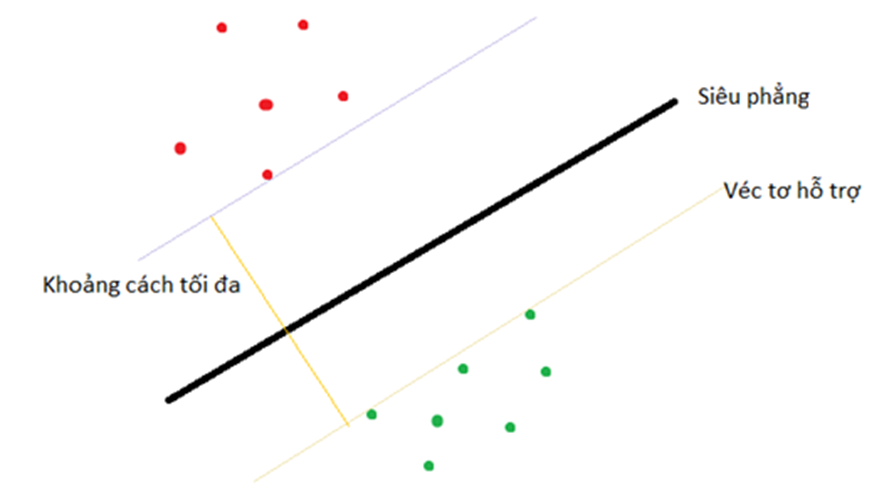
\includegraphics[width=1\linewidth]{images/svm.png}
    \caption{Tối ưu siêu phẳng sử dụng thuật toán SVM}
    \label{svm}
\end{figure}
Khoảng cách giữa mặt siêu phẳng và điểm dữ liệu gần nhất được gọi là biên. Mặt siêu phẳng tốt nhất hoặc tối ưu có thể tách riêng hai lớp là dòng có biên lớn nhất. Chỉ những điểm này có liên quan đến việc xác định hyperplane và trong việc xây dựng các điểm phân loại. Những điểm này được gọi là các vector hỗ trợ. Chúng hỗ trợ hoặc xác định hyperplane. Trong thực tế, một thuật toán tối ưu được sử dụng để tìm các giá trị cho các hệ số tối đa hóa biên. SVM có thể là một trong những phương pháp phân loại hàng đầu mạnh mẽ nhất và đáng thử trên tập dữ liệu. Cũng như hồi quy Logistic thì SVM cũng chỉ sử dụng để phân loại nhị phân. Để giải quyết vấn đề này thì có 2 phương pháp:

\begin{figure}
    \centering
    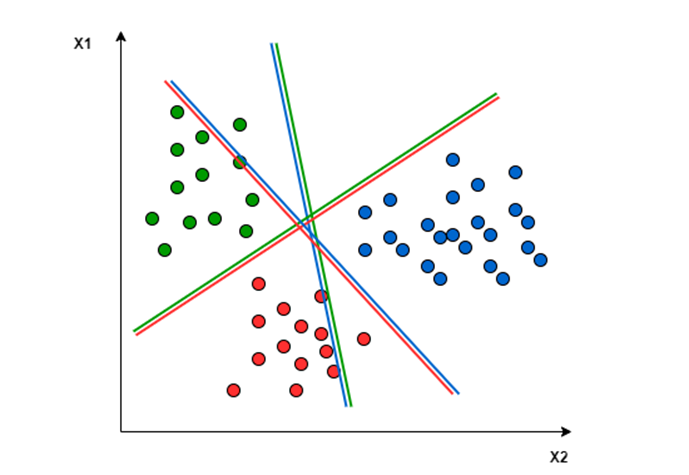
\includegraphics[width=0.6\linewidth]{images/svm_ovso.png}
    \caption{Thuật toán một với một}
    \label{svm_ovso}
\end{figure}



\begin{figure}
    \centering
    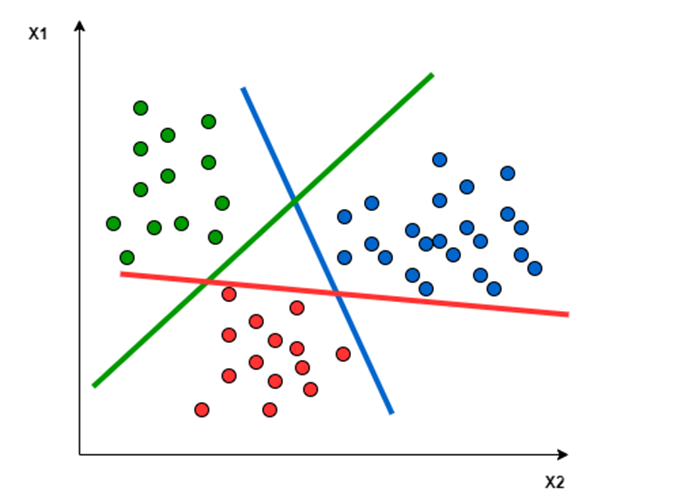
\includegraphics[width=0.6\linewidth]{images/ovsr.png}
    \caption{Thuật toán một với nhiều}
    \label{ovsr}
\end{figure}

\begin{itemize}
    \item Một với một (one vs one): Một mặt siêu phẳng được thiết lập để phân tách giữa hai lớp, bỏ qua các điểm của lớp thứ ba. Điều này có nghĩa là sự phân tách chỉ tính đến điểm của hai lớp trong sự phân tách hiện tại. Ví dụ: đường màu đỏ-xanh dương sẽ tách tối đa khoảng cách chỉ giữa các điểm màu xanh lam và màu đỏ Hình ~\ref{svm_ovso}.
    
    \item Một với nhiều (one vs rest): Cần một mặt siêu phẳng để tách biệt giữa một lớp và tất cả các lớp khác cùng một lúc. Điều này có nghĩa là sự tách biệt có tính đến tất cả các điểm, chia chúng thành hai nhóm; một nhóm cho các điểm của lớp và một nhóm cho tất cả các điểm khác. Ví dụ: đường màu sẽ tách tối đa hóa khoảng cách giữa các điểm màu lục và tất cả các điểm khác cùng một lúc Hình ~\ref{ovsr}.
\end{itemize}






\textbf{Rừng ngẫu nhiên (Random Forest - RF)}: được xây dựng trên cơ sở thuật toán Decision Tree (cây quyết định). Mỗi cây quyết định sẽ khác nhau (có yếu tố ngẫu nhiên khác nhau). Sau đó kết quả dự đoán được tổng hợp từ các cây quyết định. Trong thuật toán Decision Tree, khi xây dựng cây quyết định nếu để độ sâu tùy ý thì cây sẽ phân loại đúng hết các dữ liệu trong tập training dẫn đến mô hình có thể dự đoán tệ trên tập validation/test, khi đó mô hình bị quá khớp (overfitting).
Thuật toán Random Forest gồm nhiều cây quyết định, mỗi cây quyết định đều có những yếu tố ngẫu nhiên:
Lấy ngẫu nhiên dữ liệu để xây dựng cây quyết định.
Lấy ngẫu nhiên các thuộc tính để xây dựng cây quyết định.
Do mỗi cây quyết định trong thuật toán Random Forest không dùng tất cả dữ liệu training, cũng như không dùng tất cả các thuộc tính của dữ liệu để xây dựng cây nên mỗi cây có thể sẽ dự đoán không tốt, khi đó mỗi mô hình cây quyết định không bị overfitting mà có thế bị underfitting, hay nói cách khác là mô hình có high bias. Tuy nhiên, kết quả cuối cùng của thuật toán Random Forest lại tổng hợp từ nhiều cây quyết định, thế nên thông tin từ các cây sẽ bổ sung thông tin cho nhau, dẫn đến mô hình có low bias và low variance, hay mô hình có kết quả dự đoán tốt.
	Những kiến thức cơ bản về học máy sẽ được ứng dụng sâu trong những nghiên cứu tới đây của tác giả.

